\documentclass[11pt]{../hmcpsetrhino}
\usepackage[margin=1in]{geometry}
\usepackage{amsmath,amssymb,amsthm,enumerate,graphicx}
\renewcommand{\labelenumi}{{ \bf{(\alph{enumi})} }}
\newcommand{\ds}{\displaystyle}
\def\rcurs{{\mbox{$\resizebox{.16in}{.08in}{
\includegraphics{../ScriptR}}$}}}
\def\brcurs{{\mbox{$\resizebox{.16in}{.08in}{
\includegraphics{../BoldR}}$}}}
\def\hrcurs{{\mbox{$\hat \brcurs$}}}
\name{}
\class{Physics 151}
\assignment{Problem Set 1}
\duedate{6 September 2017}

\begin{document}
\textbf{Help}: 
%===========================================================

\begin{problem}[2.16] \\
	A long coaxial cable (Fig 2.26) carries a uniform \emph{volume} charge density $\rho$ on the inner cylinder (radius $a$), and a uniform \emph{surface} charge density on the outer cylindrical shell (radius $b$). This surface charge is negative and is of just the right magnitude that the cable as a whole is electrically neutral. Find the electric field in each of the three regions: (i) inside the inner cylinder ($s < a$), (ii) between the cylinders ($a < s < b$), (ii) outside the cable ($s <b$). Plot $|\mathbf E |$ as a function of $s$.
	$$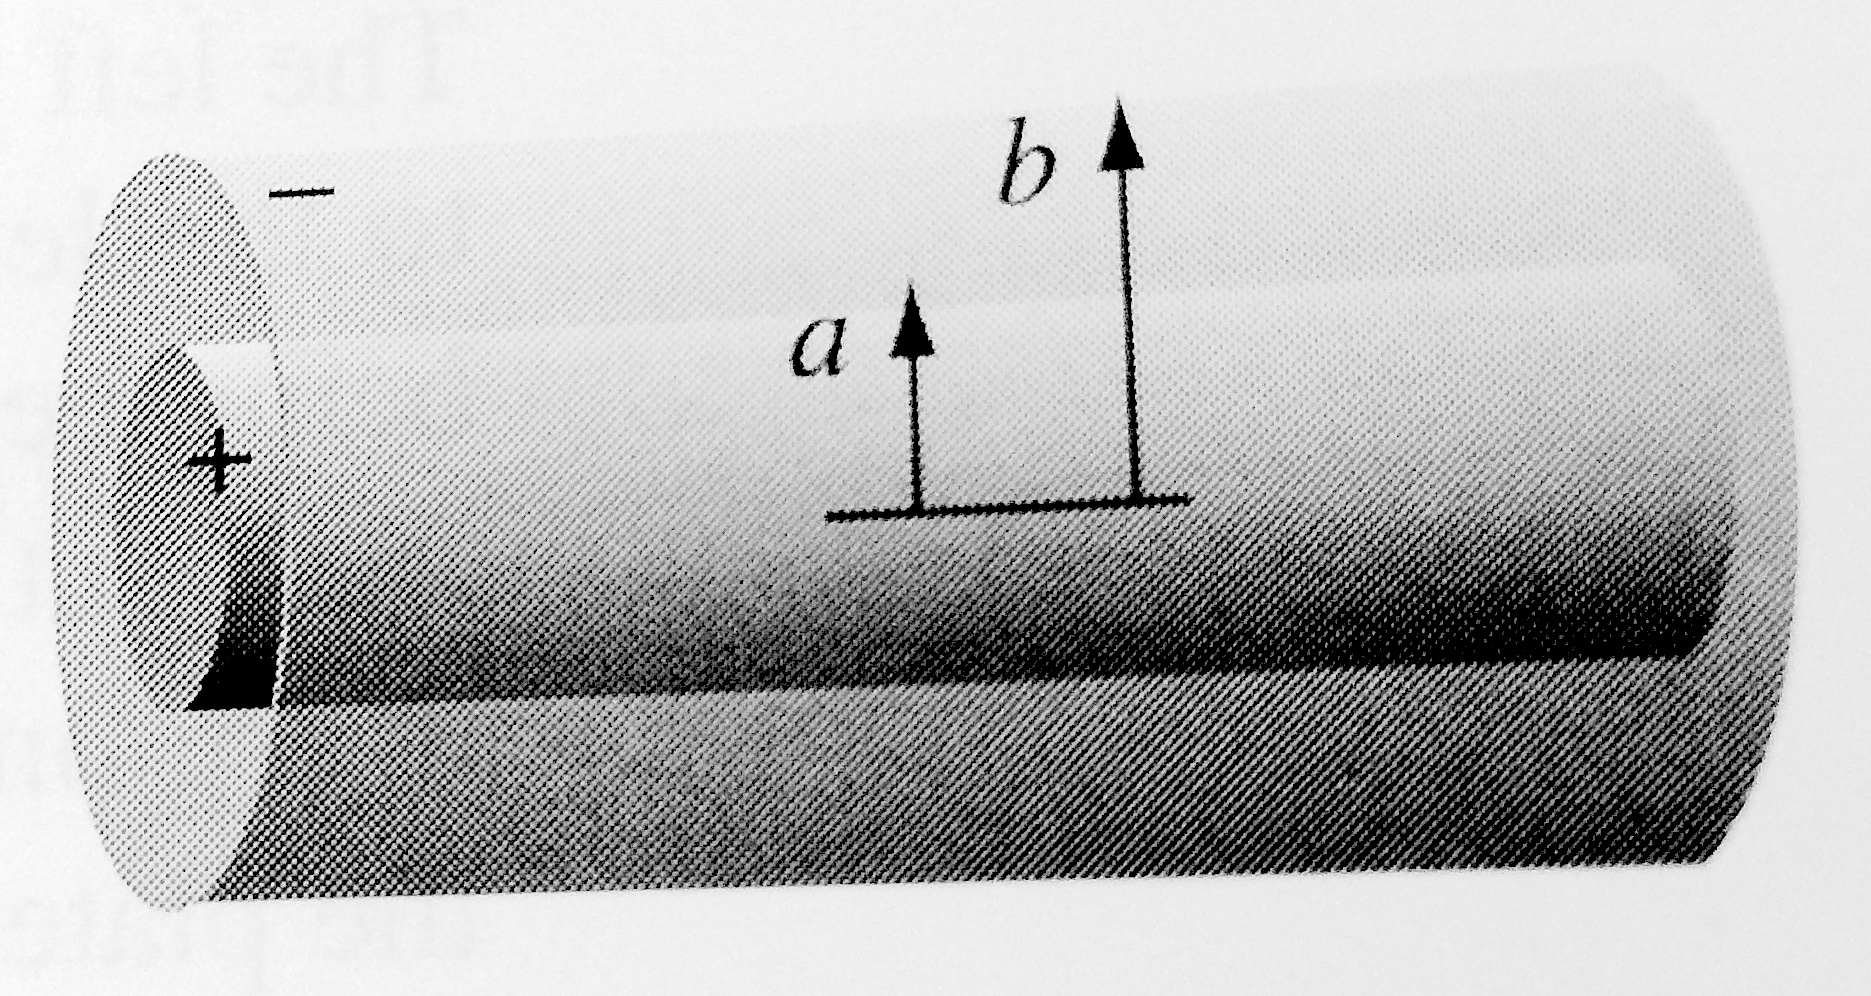
\includegraphics[scale = 0.1]{fig2-26}$$
\end{problem}

\begin{solution}
\vfill
\end{solution}

\pagebreak

%===========================================================

\begin{problem}[2.18] \\
	Two spheres, each of radius $R$ and carrying uniform volume charge densities $+\rho$ and $-\rho$, respectively, are placed so that they partially overlap (Fig 2.28). Call the vector from the positive center to the negative center $\bf d$. Show that the field in the region of overlap is constant, and find its value. [\emph{Hint}: Use the answer to Prob. 2.12.]
	$$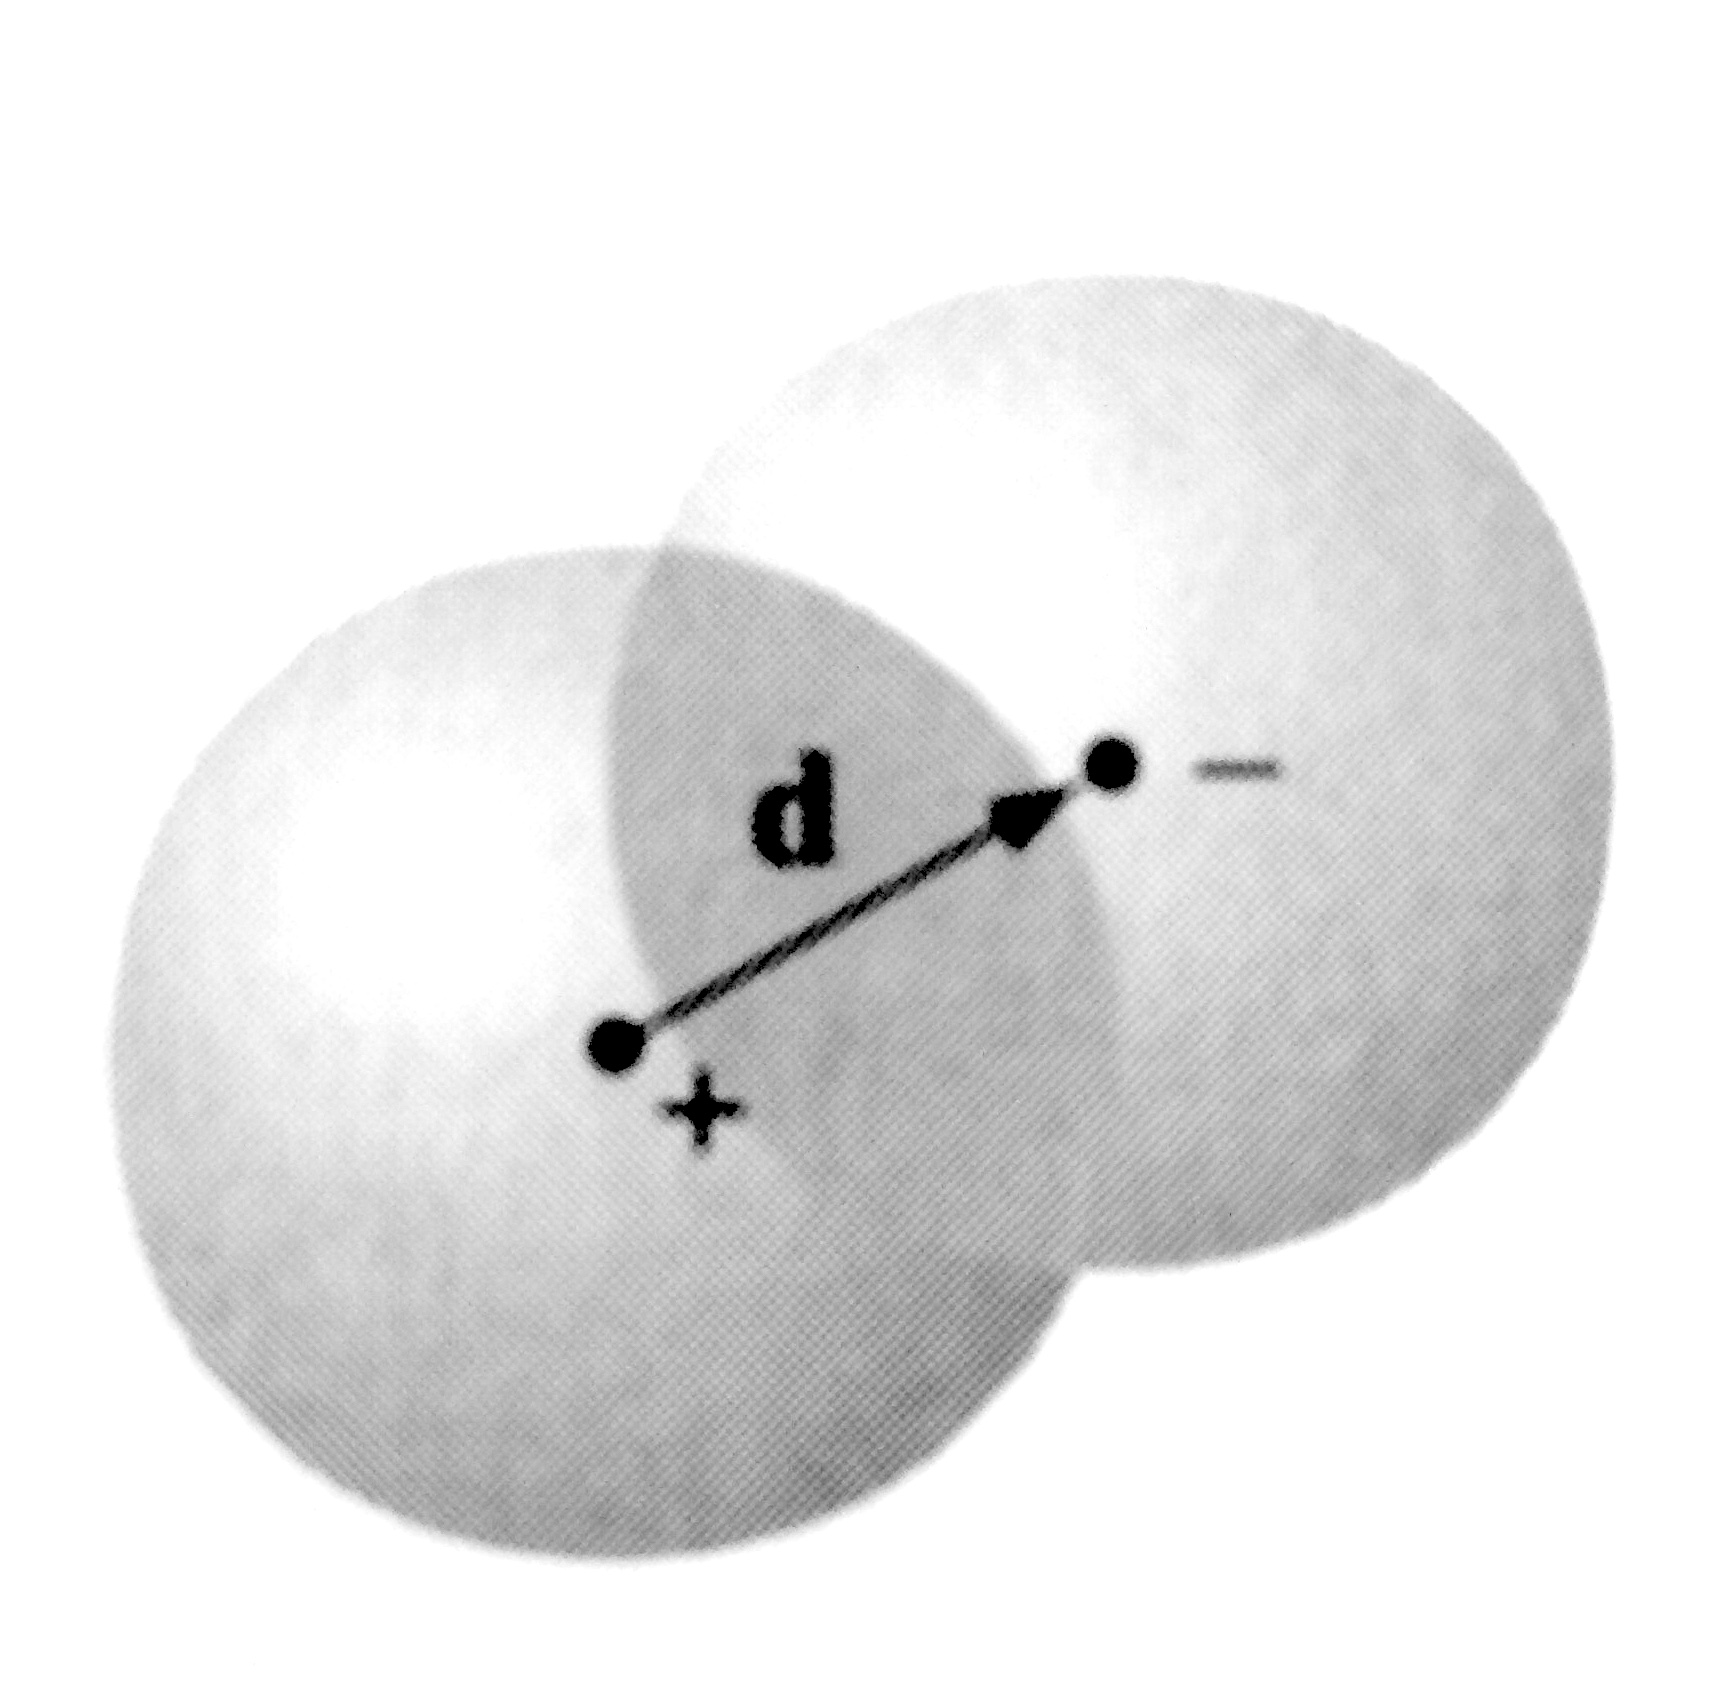
\includegraphics[scale=0.1]{fig2-28}$$
\end{problem}

\begin{solution}
\vfill
\end{solution}

\pagebreak

%===========================================================

\begin{problem}[2.26 Wolfram OK] \\
A conical surface (an empty ice-cream cone) carries a uniform surface charge $\sigma$. The height of the cone is $h$, as is the radius of the top. Find the potential difference between points $\bf a$ (the vertex) and $\bf b$ (the center of the top).
\end{problem}

\begin{solution}
\vfill
\end{solution}

\pagebreak

%===========================================================

\begin{problem}[2.60] \\
	A point charge $q$ is at the center of an uncharged spherical conducting shell, of inner radius $a$ and outer radius $b$. \emph{Question}: How much work would it take to move the charge out to infinity (through a  tiny hole drilled in the shell)? [\emph{Answer}: $(q^2/4 \pi \epsilon_0)(1/a)$]
\end{problem}

\begin{solution}
\vfill
\end{solution}

\pagebreak

%===========================================================
\end{document}

